% flashcards-title: Original and new baseline bars
% flashcards-desc: One bar has length eighty and a second has length one hundred, with the additional twenty hatched.
\documentclass[dvisvgm,tikz,border=8pt]{standalone}\usetikzlibrary{arrows.meta,patterns}

\definecolor{qraNavy}{HTML}{17324D}
\definecolor{qraBlue}{HTML}{2B6CB0}
\definecolor{qraGold}{HTML}{B7791F}
\definecolor{qraPale}{HTML}{EAF2F8}
\definecolor{qraGray}{HTML}{5C6773}

\tikzset{
  qra axis/.style={draw=qraNavy, line width=1.2pt},
  qra tick/.style={draw=qraNavy, line width=1pt},
  qra guide/.style={draw=qraGray, densely dashed, line width=0.8pt},
  qra counter/.style={circle, draw=qraNavy, fill=qraPale, line width=0.9pt, minimum size=7mm, inner sep=0pt},
  qra label/.style={font=\sffamily\bfseries, text=qraNavy},
  qra small label/.style={font=\sffamily, text=qraNavy},
}

\begin{document}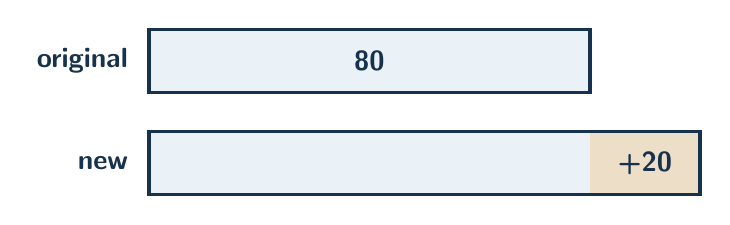
\begin{tikzpicture}[x=.07cm,y=1cm]\fill[qraPale](0,1.3)rectangle(80,2.1);\draw[qra axis](0,1.3)rectangle(80,2.1);\node[qra label,left=4pt]at(0,1.7){original};\node[qra label]at(40,1.7){80};\fill[qraPale](0,0)rectangle(80,.8);\fill[fill=qraGold!25](80,0)rectangle(100,.8);\draw[qra axis](0,0)rectangle(100,.8);\node[qra label,left=4pt]at(0,.4){new};\node[qra label]at(90,.4){+20};\end{tikzpicture}\end{document}
